\section{EMBERS Successes and Misses}
Next, we detail
some of the successful as well as not so successful forecasts made by EMBERS over
the past few years in Latin America.
\subsection{Successful Forecasts}
\subsubsection*{Brazilian Spring (June 2013)}
These protests were the largest and most
significant protests in Brazil's recent history and caught worldwide
attention. Millions of Brazilians took part in these demonstrations,
also known as the Brazilian Spring or the Vinegar Movement (inspired
from the use of vinegar soaked cloth by demonstrators to protect
themselves from police teargas). These protests were
sparked by an increase in public transport fares from $R\$3$
to $R\$3.20$ by the government of President Dilma Rousseff.

As shown in Figure.~\ref{fig:brazilJune13} EMBERS, while missing the initial uptick,
forecast the increase in the order-of-magnitude of protest events
during the Brazilian Spring and also captured
the spatial spread in the events, in addition to forecasting that this event
will span the broad Brazilian general population (as opposed to being confined to
specific sectors).

\begin{figure}[H]
\centering
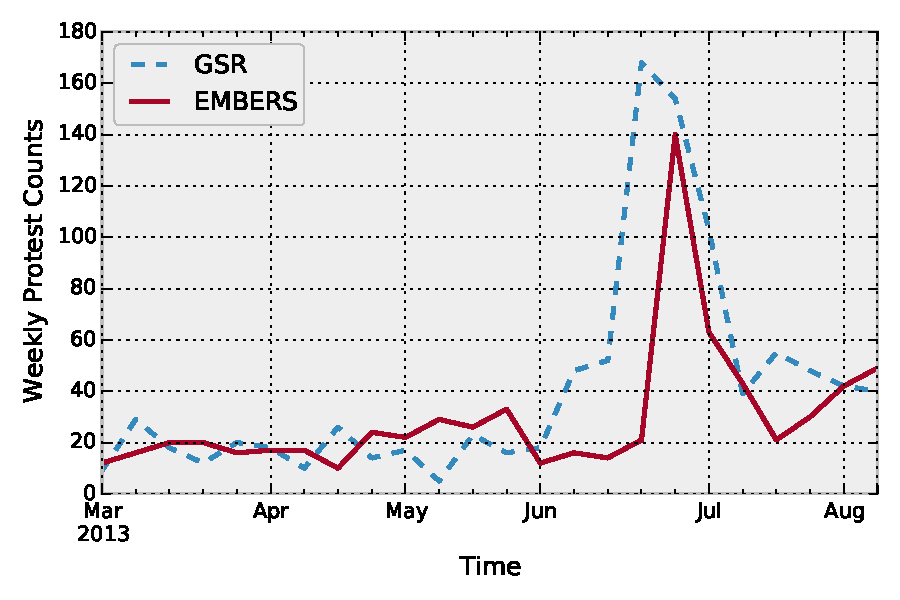
\includegraphics[width=.8\columnwidth]{cu/brazilJune13}
\caption{EMBERS performance during the Brazilian Spring (June 2013.)}
\label{fig:brazilJune13}
\end{figure}

Around 68\% of EMBERS alerts during this period originated from
the planned protest model.
This is due to the fact that
social networking
platforms (Twitter and Facebook) as well as conventional news media played a key
role in organization of these uprisings. Although initial protests were
primarily due to the bus fare increases, they quickly morphed into
more broader dissatisfaction to include wider issues such as
government corruption, over-spending, and police brutality. The
demonstrators also made calls for political reforms. In response, President
Rousseff proposed a plebiscite on widespread political reforms in
Brazil (but this was was later abandoned). Through its dynamic query expansion model,
EMBERS was able to capture such discussions on Twitter
(see Figure.~\ref{fig:brazilJune13_wordCloud}), and tracked their evolution as events
unfolded through June.

\begin{figure}[H]
\centering
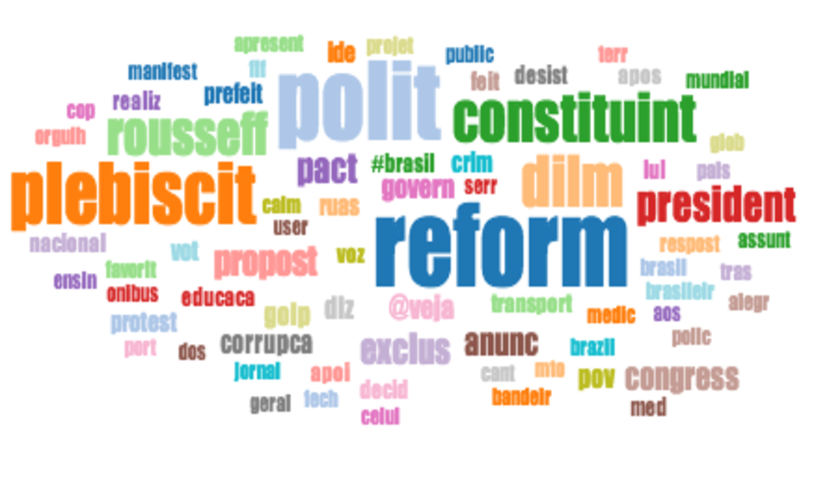
\includegraphics[width=.8\columnwidth]{cu/brazilJune13_wordCloud}
\caption{Word cloud representing tweets identified by EMBERS dynamic query expansion model.}
\label{fig:brazilJune13_wordCloud}
\end{figure}

The protests intensified in late June (see Figure.~\ref{fig:brazilJune13}), which were
forecast correctly by EMBERS, and these events
also coincided with FIFA 2013 Confederation Cup matches. We believe this was an important factor in helping
the protests gain momentum,
as the events were covered by international media. A majority of protests
occurred in the cities that were hosting FIFA soccer matches.
EMBERS issued most of its alerts for these host cities (see Figure
~\ref{fig:brazilJune13_map}), viz.
Rio de Janeiro, São Paulo,
Belo Horizonte, Salvador, and Porto Alegre,
among others. For example, on 27th June during the Confederations Cup
semi-final in Fortaleza, around 5000 protesters clashed with the police
near the Castelao stadium. In this case EMBERS had forecast an alert the
day before. Later on the 30th of June, when the last games of the
confederation cup took place in Rio de Janeiro and Salvador, they
were plagued by mass protests as well; EMBERS predicted these events and
submitted multiple alerts for Rio for the 28th and 29th June and one for
Salvador for 29th June.

\begin{figure}[H]
\centering
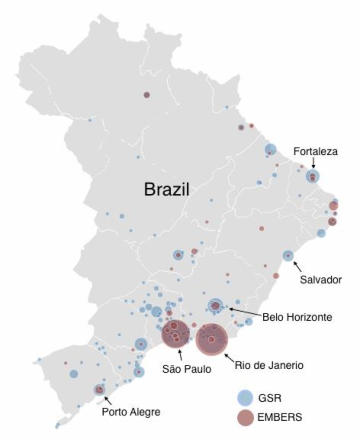
\includegraphics[height=.6\columnwidth]{cu/brazilJune13_map}
\caption{Geographic overlap of protest events (from the GSR) and EMBERS
alerts for Brazil during June 2013.}
\label{fig:brazilJune13_map}
\end{figure}

\subsubsection*{Venezuelan Protests (Feb-March 2014)}
Early 2014 Venezuela started experiencing a situation of turmoil with a 
large portion of its population protesting due to insecurity, inflation 
and shortage of basic goods. This period saw one of the highest levels of
civil disobedience in Venezuela with protests beginning in January with the murder
of a former Miss Venezuela. However, the protests started gaining more importance
 and turned violent and more frequent with students joining the movement following an
attempted rape of a student on campus in San Cristobal. EMBERS captured
some of these first `calls to protest` at San Cristobal and its nearby surrounding areas
 and correctly forecast the population (Education) and that the protests would turn violent. 
A majority of the protesters were demanding that president Nicolas Maduro step down owing
to the poor economic policies and widespread corruption. EMBERS was capable of capturing 
that the reason behind the protests were mainly against government policies with corruption being  
a major theme.The EMBERS models working on twitter were also clearly able to identify some of major 
leaders involved in the protest such as the major opposition leader Leopoldo Lopez.
Though the events mainly started off from San cristobal it spread widely throughout the country, EMBERS
captured this spillover very well as shown in Fig.~\ref{fig:venezuelaMap}.The Fig.~\ref{fig:venezuelaMarch14}
shows how EMBERS closely forecast the spike in the number of events  during this period.
%Over the next
%days, EMBERS closely forecast the spike in the number of events as shown
%in Fig.~\ref{fig:venezuelaMarch14} and the spread
%of the protests to additional cities as shown in
%Fig.~\ref{fig:venezuelaMap}.
%The protests were peaceful with a majority of
%the protesters demanding the president Nicolas Maduro to step down.
\begin{figure}[H]
\centering
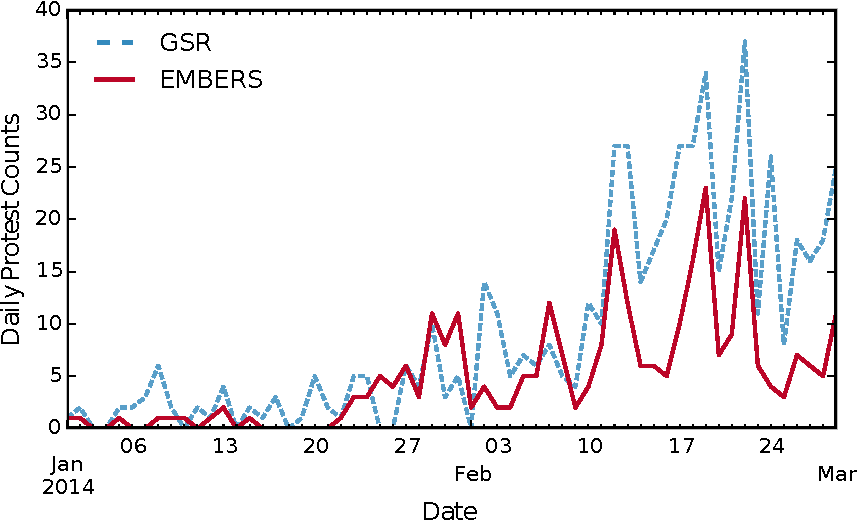
\includegraphics[width=.8\columnwidth]{cu/venezuelaFeb14}
\caption{EMBERS performance during the Venezuelan student protests (Feb-Mar 2014).}
\label{fig:venezuelaMarch14}
\end{figure}

\begin{figure}[H]
\centering
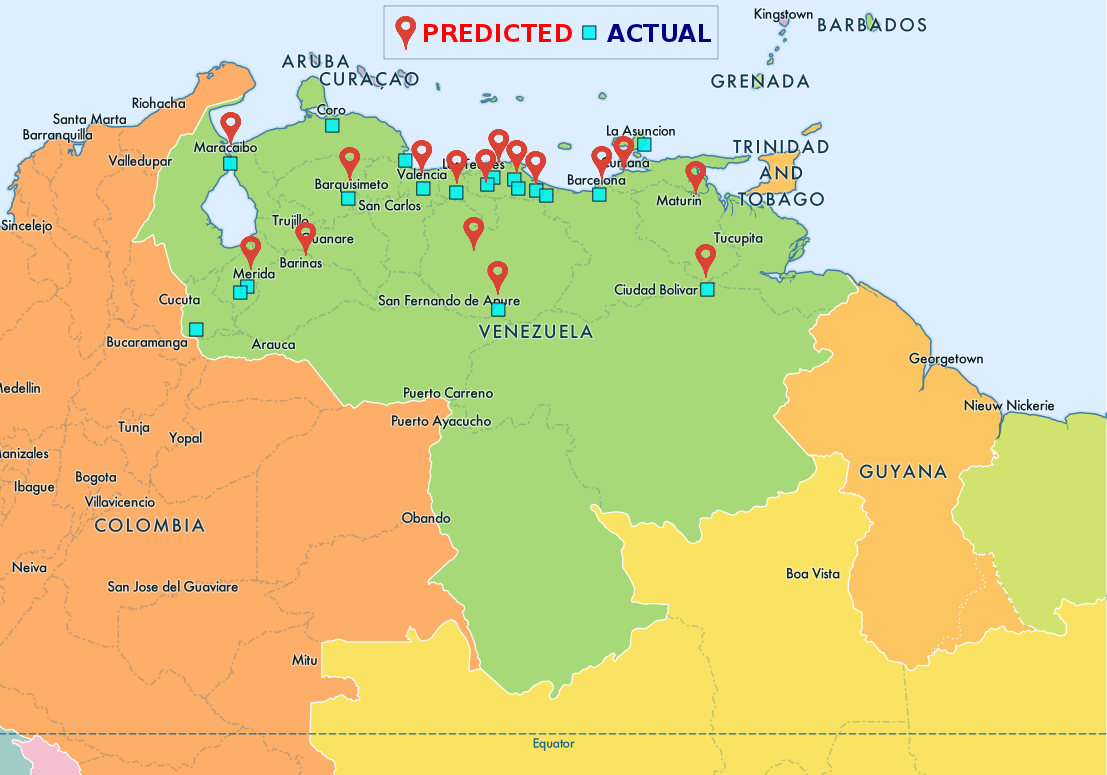
\includegraphics[width=.6\columnwidth]{cu/venezuelaMap}
\caption{Geographical spread of protests (and forecasts) during
Venezuelan student protests (Feb-Mar 2014).}
\label{fig:venezuelaMap}
\end{figure}

\subsubsection*{Mexico Protests (Oct 2014)}
\narenc{First, write one para about what these protests are about.}
Late September 2014, there were some peaceful protests by students from Ayotzinapa
in Mexico against discriminatory hiring practices for teachers. During this protest,
police opened fire on the students killing around three and about 43 went missing. This poor
handling of the protest by the Mexican government caused widespread demonstrations throughout
the country over the next few months in support of the families of the 43 missing students.
A lot of these protests were violent in nature with demonstrators expressing extreme
dissatisfaction against the government and president Pena Nieto. EMBERS, as shown in Fig.~\ref{fig:mexicoOct14} 
forecast an uptick in Mexico protests during early October 2014 with a lead time of about three days.
It also generated  a series of alert spikes coinciding with the first
large-scale nationwide protests between October 5th and 8th.
Figure.~\ref{fig:mexicoTimeline} provides a timeline of GSR events and
EMBERS alerts for Mexico during this period. This figure provides a detailed
comparison of the continuous stream of alerts produced by EMBERS during this period with how
the actual events unfurled in the real world.


\narenc{Say more about this timeline,
a few more sentences.}

\begin{figure}[H]
\centering
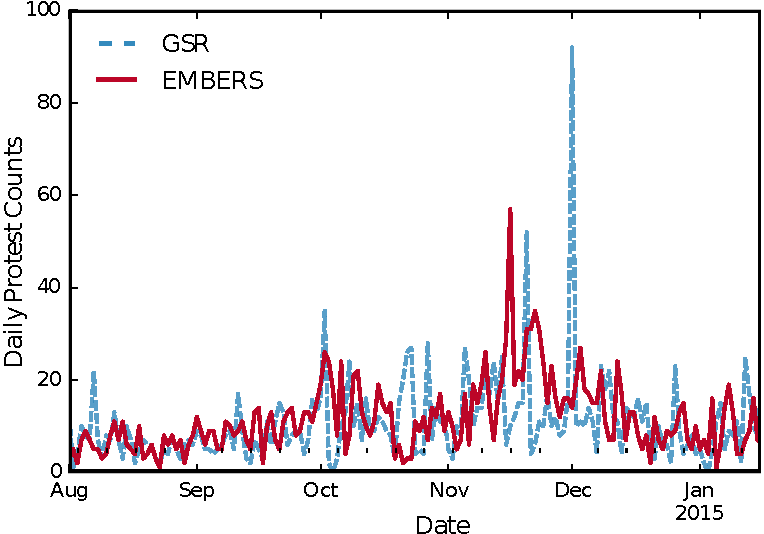
\includegraphics[width=.8\columnwidth]{cu/mexicoOct14}
\caption{EMBERS performance during Mexico protests (Oct 2014).}
\label{fig:mexicoOct14}
\end{figure}

\begin{figure}[H]
\centering
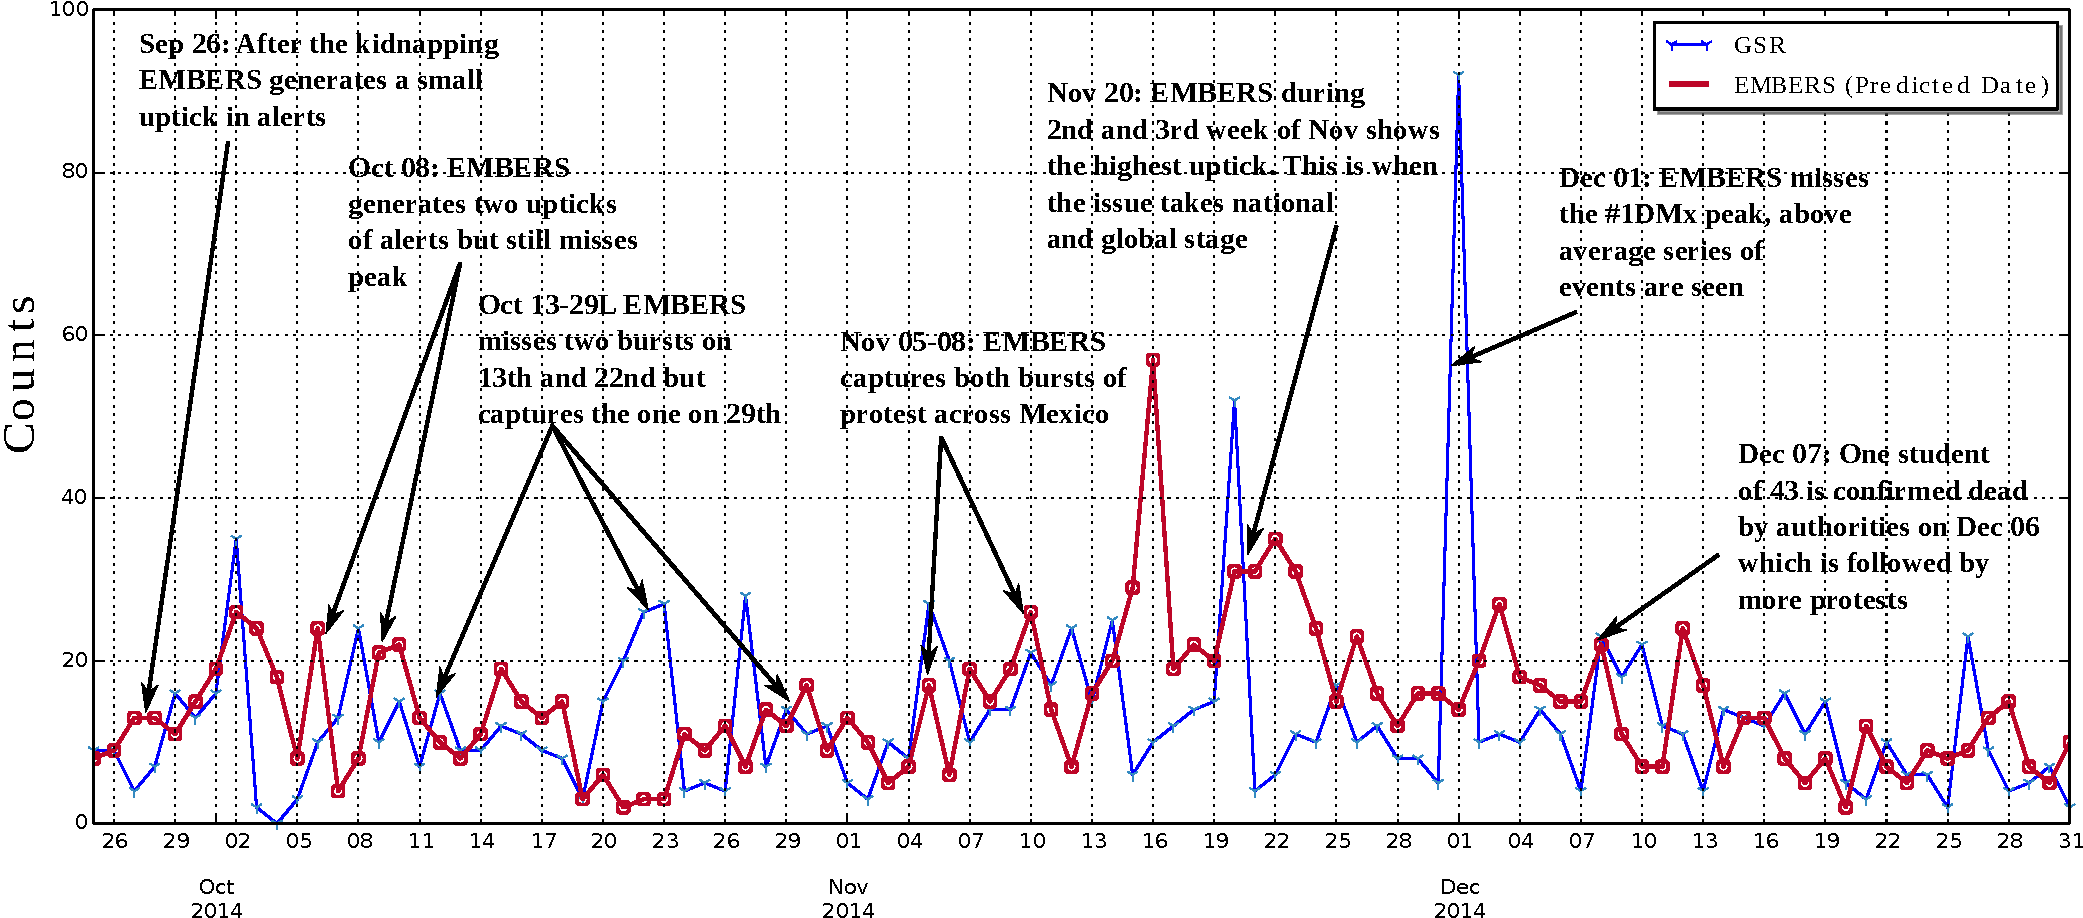
\includegraphics[width=\columnwidth]{cu/mx_timeline}
\caption{Timeline of Mexico protests, showing the correspondence
between counts of GSR events and EMBERS alerts on a daily basis.}
\label{fig:mexicoTimeline}
\end{figure}

\subsubsection*{Colombia Protests (Dec 2014 to March 2015}
\narenc{First one paragraph about what these protests are.}
Colombia witnessed two different significant protests during this period, one during late december 2014 
and the other during February 2015. Towards the end of 2014 the colombian government were on the process
of moving forward with peace negotiations to end 50 years of conflict with the Revolutionary Armed Forces 
of Colombia (FARC). With the FARC rebels having been associated with various acts of terror like extortion, armed conflict,
kidnapping, ransom, illegal mining etc., for a long period, the people of colombia gathered in huge numbers
 to protest against possible amnesty for the FARC rebels.EMBERS successfully forecast the uptick in the number of events during the
middle of December 2014 as indicated in Fig.~\ref{fig:colombiaDec14}. The figure also shows the increase in protest counts
during February 2015 though in this case EMBERS over-predicted the counts. The protests in February 2015
were mainly by led by truckers union demanding better freight rates, labor rights and against high fuel prices.
The truckers extended for about a month and caused huge losses of about \$300 milliion to the colombian economy.
EMBERS picked up on the truckers protests right from the beginning but was wrong in over estimating the numbers during 
February 11-12.
%The increase in protest counts during Feb 2015 was
%caused by a truckers' strike against fuel price increases.

\begin{figure}[H]
\centering
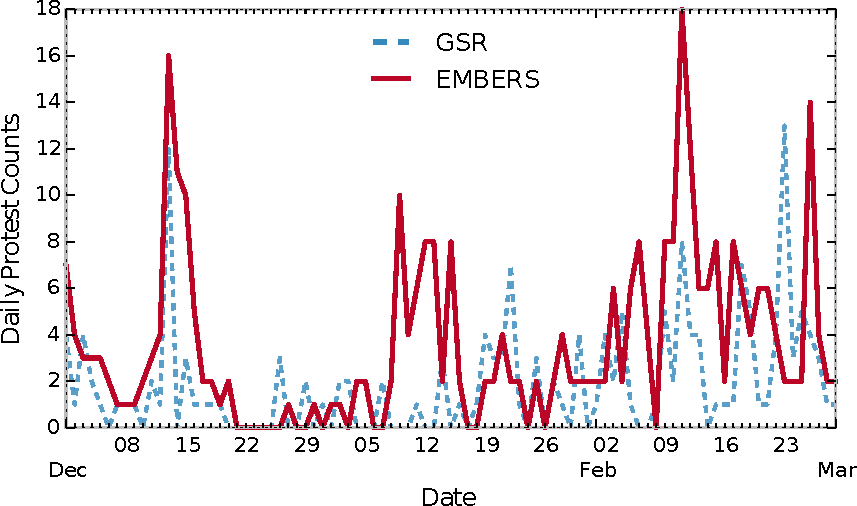
\includegraphics[width=.8\columnwidth]{cu/colombiaDec15}
\caption{Colombia Protests \narenc{rewrite caption similar to previous ones.}}
\label{fig:colombiaDec14}
\end{figure}

\subsubsection*{Paraguay Protests (February 2015)}
\narenc{First describe what these protests are about.}
The February 2015 protests in Paraguay were mainly carried out by peasants
against the actions of the President Horacio Cartes.The protests were carried out after 
president Horacio's public revelation that he had opened two private swiss bank accounts.
The protests also had a historical significance. It was also being carried out as a tribute 
to peasant leaders and activists who were murdered. The peasants also protested 
against the introduction of the new public-private partnership law.

EMBERS forecast the uptick in number of protest events in Paraguay during mid
February 2015 as shown in Fig.~\ref{fig:paraguay15}.

\begin{figure}[H]
\centering
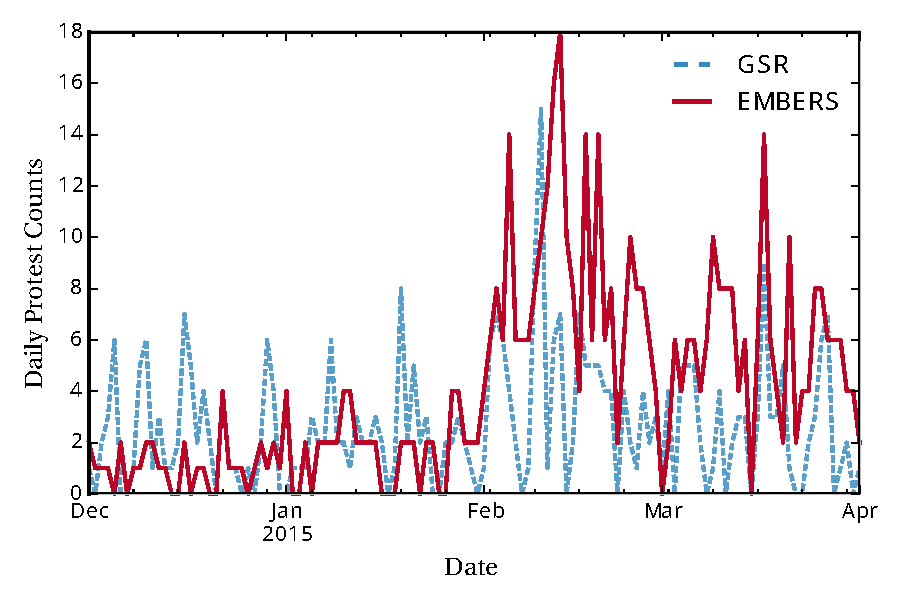
\includegraphics[width=.8\columnwidth]{cu/paraguayFeb15}
\caption{Paraguay Protests \narenc{rewrite caption similar to previous ones.}}
\label{fig:paraguay15}
\end{figure}

\subsection{EMBERS Misses}
Next, we outline specific large-scale events that
EMBERS failed to forecast accurately, along with a discussion of underlying
reasons.

\subsubsection{Brazilian Protests (March 2015)}
\narenc{First, explain what these protests are about.}
The protests were mainly targeted against president Dilma Rousseff due to
increasing corruption.
While EMBERS accurately predicted that there
will be an increase in the rate of events it failed to
capture the true counts.

During this period there was a significant architectural change in the
EMBERS processing pipeline. EMBERS had moved to the Heideltime temporal
tagger from the previously used TIMEN temporal tagger due to
Heideltime's support for more languages and an active development cycle as
opposed to TIMEN. \narenc{Find some way to mention temporal tagging somewhere
in the background section, so it doesn't appear so sudden here.}
\narenc{Also give citations for TIMEN and Heideltime.}
Heideltime had no support for Portuguese (the primary
language used in Brazil) and the EMBERS software development team had extended Heideltime to
support Portuguese by translating the underlying
resources for Spanish to Portuguese. As we learnt subsequently,
the simple translation of rules from Spanish to Portuguese
was not sufficient and this affected the recall of one of the key models
for Brazil, viz. the planned protest model. Since the planned protest model relies
almost exclusively on the quality of information (specifically, date) extraction from text,
its performance significantly deteriorated. This was subsequently corrected for the future.

\begin{figure}
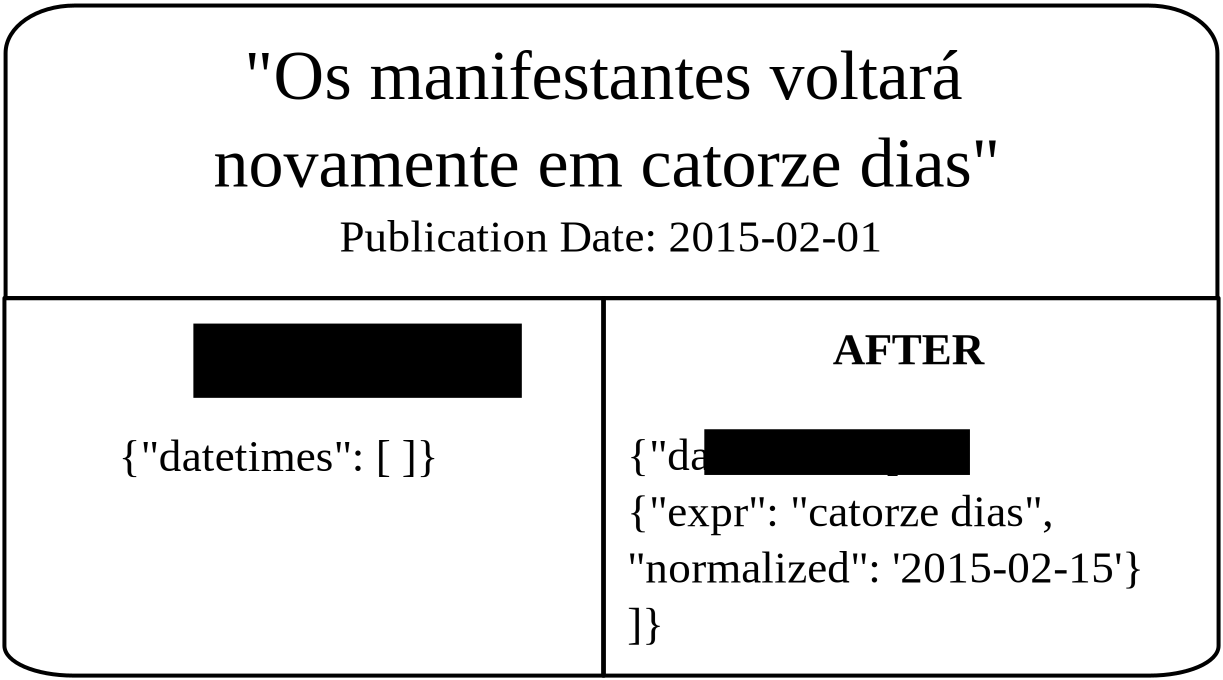
\includegraphics[width=\columnwidth]{cu/heideltime}
\caption{Example showing the improvements after heideltime improvement}
\label{fig:heideltime}
\end{figure}


\begin{figure}[H]
\centering
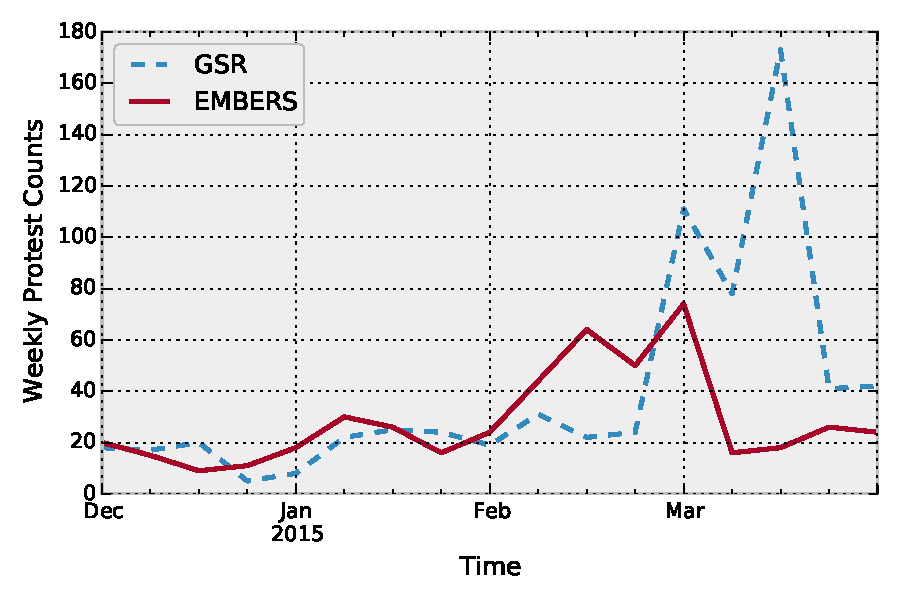
\includegraphics[width=.8\columnwidth]{cu/brazilMarch15}
\caption{Brazil 2015 Protests}
\label{fig:brazilSpring}
\end{figure}

\subsubsection{\it Mexico Protests (Dec 2014)}
During Dec 2014, people turned out in huge numbers in different cities of Mexico demanding
President Pena Nieto`s ouster. \narenc{Say more.}
EMBERS missed the huge single day spike on December 1st when
EMBERS predicted nationwide events for December 1st but failed to
capture the its spread.  \narenc{This previous sentence does not parse.
Did it miss the spike, or did it predict it correctly? Fix it.}
December 1st was picked by the protesters due to
its historical significance. This was the day when President Pena Nieto was sworn
in as President in 2012 amidst much controversy and opposition from
many specific constituent groups. A specific reason why EMBERS missed this forecast
was its inability to extract dates mentioned using Twitter lingo such as {\bf \#1Dmx}.

\subsubsection{Brazilian Spring Onset}
\narenc{Refer back to the old Brazilian Spring figure. Say as mentioned earlier, while we forecast
the duration and details of it, we missed the onset of it. Say some more about it. This is an event that
we should not have any excuse for. Point them to look at the limitations section.}

\section{Ablation Testing}
\narenc{Put the Twitter removal figure here. and discuss.}
\begin{figure}
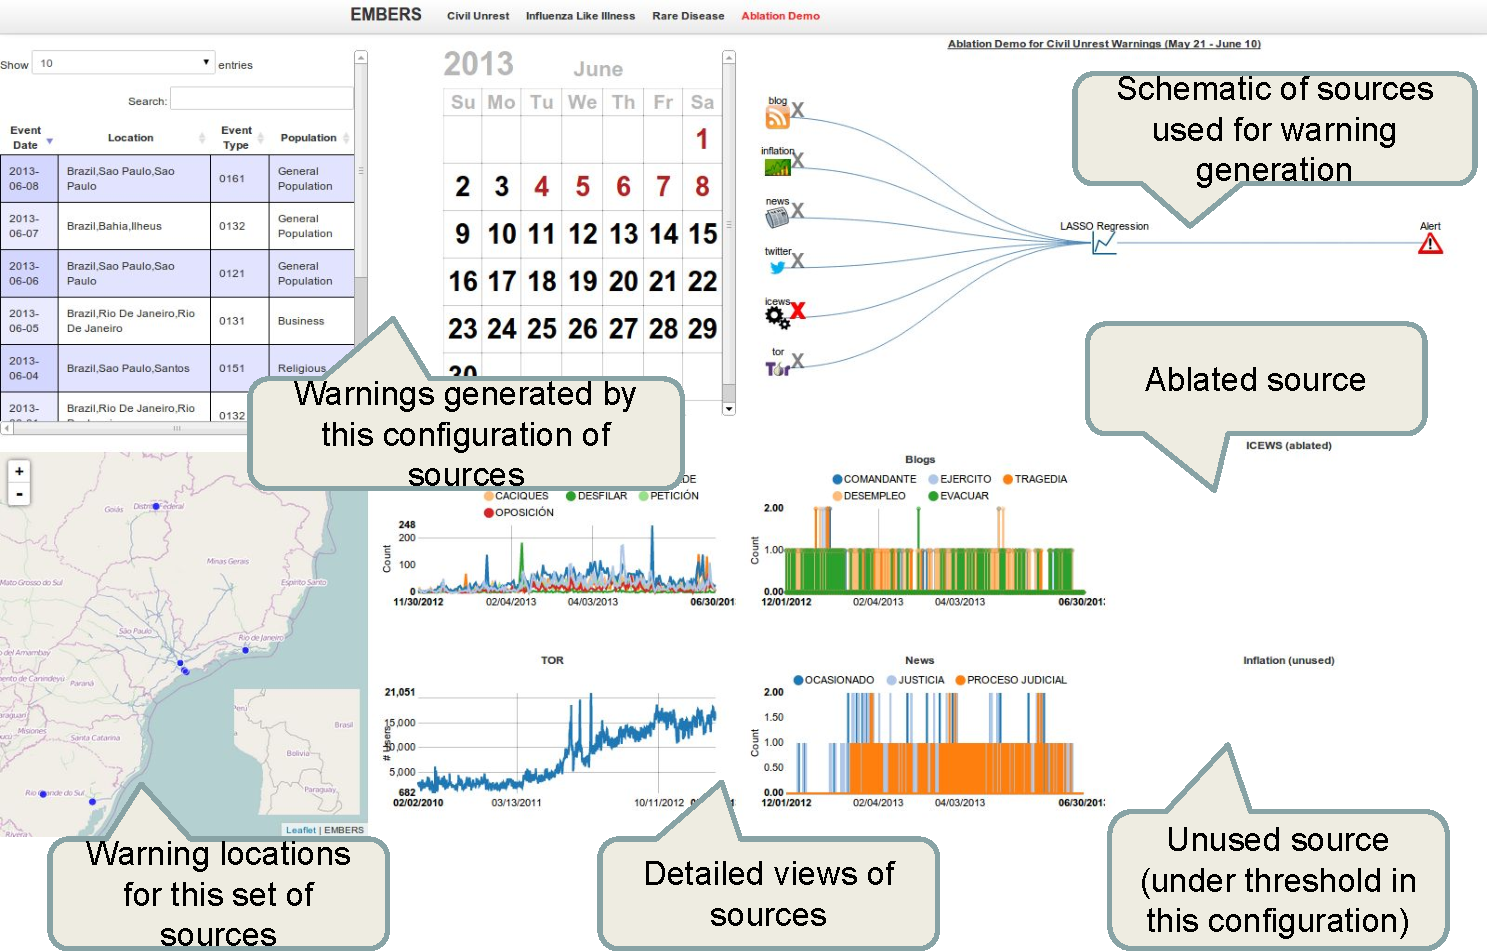
\includegraphics[width=\columnwidth]{figures/cu/ablation.pdf}
\caption{EMBERS visualization on Ablation testing}
\label{fig:ablation}
\end{figure}
\section{Forecasting Surprising Events}

%\begin{table}
%\caption{Comparison of performance metrics with and without social media sources. Social Media sources contributes a lot towards recall but loses out on
%lead-time.}
%\label{tb:ablation_twitter}
%\begin{tabular}{|c|c|c|c|c|}
%\hline
%Data Source          & Quality-Score & Lead-time & Precision & Recall \\
%\hline
%Social Media Sources & \cellcolor[red]{.16} -16.48\% & \cellcolor[red]{.55} -55\% & \cellcolor[green]{.35} +35\% & \cellcolor[red]{.14} -14\% \\
%%Social Media Sources & \cellcolor[red]{.16} -16.48\% & \cellcolor{red!55} -55\% & \cellcolor{green!35} +35\% & \cellcolor{red!14} -14\% \\
%\hline
%Non-Social Media Sources & \cellcolor{green!10} +8.42\% & \cellcolor{green!40} +30\%  & \cellcolor{green!60} +79\% & \cellcolor{red!30} -33\% \\
%\hline
%\end{tabular}
%\end{table}
\begin{table}
%\small
\caption{Comparison of performance measures under ablation testing.
Social media sources contribute toward recall but, due to their noisy
nature, lower other measures of performance.}
\label{tb:ablation_twitter}
\vspace{-3mm}
\resizebox{\columnwidth}{!}{
\begin{tabular}{|L|c|c|c|c|}
\hline
Data Source          & Quality-Score & Lead-time & Precision & Recall \\
\hline
Removing news and blogs & -16.48\% &-55\% &+35\% &-14\% \\
\hline
Removing social media & +8.42\% & +30\%  &+79\% &-33\% \\
\hline
\end{tabular}
}
\end{table}

The GSR contains a mix of everyday, mundane, protests as well as surprising events such as the Brazilian Spring.
We aimed to ascertain the relative ease of forecasting each class of events
with respect to a simple baserate model.

The baserate model generates alerts using the rate of occurrence of events in the past three months.
\narenc{Talk about Ecuador slides.}

To define surprising events,
we employed a maximum entropy approach. For this purpose, each event is assumed
to be describable
in terms of three dimensions: country, population and event type. The GSR can then be conceptualized
as the cube shown in Fig.~\ref{fig:maxent_model}. We infer a maximum entropy distribution conditioned on the marginals
induced by the cube using iterative proportional fitting~\cite{bishop2007discrete}, as shown in \narenc{Put the algo below in some nice box.}

\begin{enumerate}
\item Once the marginals are identified, elementary cells are replaced by 1; $\widehat{m}^{(0)}_{ijk}=1$
\item After initialization, the following three-step iterative cycle is performed till a satisfactory stopping goal is achieved:
$$\widehat{m}^{(c+1)}_{ijk} = \widehat{m}^{(c)}_{ijk}\frac{x_{ij+}}{\widehat{m}^{(c)}_{ij+}}$$
$$\widehat{m}^{(c+2)}_{ijk} = \widehat{m}^{(c+1)}_{ijk}\frac{x_{i+k}}{\widehat{m}^{(c+1)}_{i+k}}$$
$$\widehat{m}^{(c+3)}_{ijk} = \widehat{m}^{(c+2)}_{ijk}\frac{x_{+jk}}{\widehat{m}^{(c)}_{+jk}}$$
where $c$ refers to iteration cycle and `+' refers to summation over a dimension.
\item The procedure stops if either the desired convergence of $\delta < 0.0001$ is achieved or the maximum number of iterations are reached.
\end{enumerate}

\narenc{The procedure above makes no sense - the symbols are not defined at all.}

\begin{figure}[H]
\centering
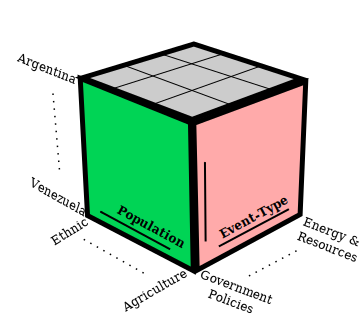
\includegraphics[width=.7\columnwidth]{cu/maxent_model}
\caption{Modeling the maxent distribution of civil unrest counts to identify surprising events.}
\label{fig:maxent_model}
\end{figure}

Every month, events from the last three months of the
GSR is used to populate the underlying cube of counts and the iterative proportional fitting procedure is
used to estimate the maxent values for each cell. The resultant sample counts are then scaled to
match the observed number of GSR events in the current month. The cell-wise difference between the inferred
maxent distribution and the observed GSR is computed and all cells with significance greater than five standard
deviations are classified as containing surprising events. In essence, this approach takes the GSR as input and
creates a truncated GSR against which we can evaluate EMBERS (and the baserate model).

\begin{table}
\caption{Surprising events inferred by maxent analysis.}
\renewcommand{\arraystretch}{1.1}
\vspace{-3mm}
 \centering
 \begin{tabular}{|l|l|m{5cm}|}
 \hline
May '13  &  Colombia	 &  Nationwide protests against administrative policy changes regarding the
Youth in Action program and social security pension \\ \hline
Jun '13  &  Brazil  &  Brazilian Spring \\ \hline
Jul '13  &  Brazil  &  Brazilian Spring \\ \hline
Sep '13  &  Mexico  &  Nationwide protests against education and energy reforms \\ \hline
Oct '13  &  Mexico  &  Nationwide protests against education and energy reforms \\ \hline
Oct '13  &  Uruguay  &  Nationwide protests demanding increase in minimum wage \\ \hline
Feb '14  &  Venezuela	  &  Venezuelan Student Protests \\ \hline
Mar '14  &  Venezuela  &  	Venezuelan Student Protests \\ \hline
May '14  &  Brazil  &  Nationwide demonstrations in response to the 2014 FIFA World Cup and other social issues \\ \hline
Jun '14  &  Brazil  &  Nationwide demonstrations in response to the 2014 FIFA World Cup and other social issues \\ \hline
Aug '14  &  Argentina	  &  Nationwide protests against drops in wages, employment, and rising inflation \\ \hline
Sep '14  &  Ecuador  &  Nationwide protests to demand changes in labor policies \\ \hline
Oct '14  &  Mexico  &  Nationwide protests after the discovery of mass graves of kidnapped students  \\ \hline
\end{tabular}
%\vspace{-5mm}
\label{tab:maxentEvents}
\end{table}

In Table~\ref{tab:maxentEvents} we present several inferred events in Latin America from our maximum entropy
filter.
For all these events, we compare the recall of both EMBERS and baserate model in Fig.~\ref{fig:maxent}.
It is clear that EMBERS is able to forecast these significant upticks consistently.

\begin{figure}[H]
\centering
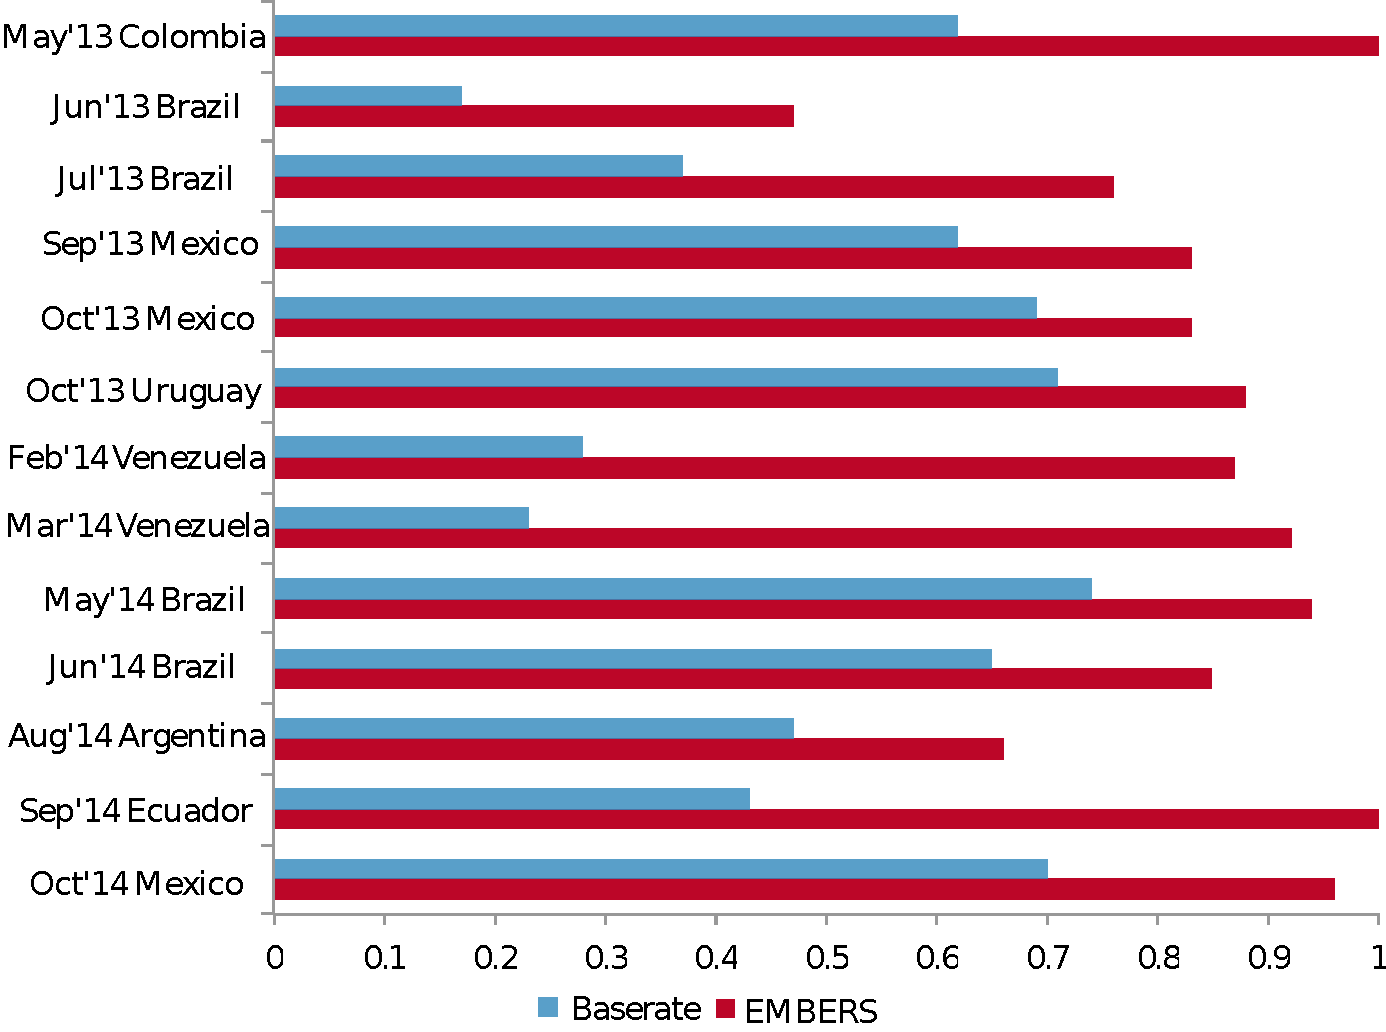
\includegraphics[width=.99\columnwidth]{cu/maxent}
\caption{Performance of EMBERS vs a baserate model for surprising events.}
\label{fig:maxent}
\end{figure}
